\documentclass[11pt,letterpaper]{article}

% ---- Packages ----
\usepackage[margin=1in]{geometry}
\usepackage{amsmath,amssymb,amsthm}
\usepackage{graphicx}
\usepackage{hyperref}
\usepackage{xcolor}
\usepackage{booktabs}
\usepackage{enumitem}
\usepackage{caption}
\usepackage{subcaption}
\usepackage{listings}
\usepackage{fancyhdr}
\usepackage[section]{placeins}   % prevent floats from drifting past section boundaries
\usepackage{float}               % provides [H] placement specifier
\usepackage{pifont}              % for checkmarks and crosses
\newcommand{\cmark}{\ding{51}}
\newcommand{\xmark}{\ding{55}}
% biblatex removed: using \thebibliography for portability (no .bib file needed)

% ---- Colors ----
\definecolor{codegreen}{rgb}{0.25,0.78,0.54}
\definecolor{codegray}{rgb}{0.5,0.5,0.5}
\definecolor{codebg}{rgb}{0.96,0.97,0.98}

% ---- Code style ----
\lstset{
  language=Python,
  basicstyle=\small\ttfamily,
  backgroundcolor=\color{codebg},
  keywordstyle=\color{blue!70!black},
  commentstyle=\color{codegray},
  stringstyle=\color{codegreen},
  breaklines=true,
  frame=single,
  framerule=0.4pt,
  rulecolor=\color{gray!30},
  numbers=none,
  xleftmargin=6pt,
  xrightmargin=6pt,
}

% ---- Header ----
\pagestyle{fancy}
\fancyhf{}
\rhead{\textit{Normalizing Flows for Bayesian Inference}}
\lhead{\textit{Mingarelli}}
\cfoot{\thepage}

% ---- Title ----
\title{Normalizing Flows for Bayesian Inference:\\
An Interactive Tutorial}
\author{Chiara Mingarelli\\
\small Department of Physics, Yale University\\
\small Center for Computational Astrophysics, Flatiron Institute\\
\small \texttt{chiara.mingarelli@yale.edu}
\and
Abigail Moran\\
\small Department of Physics, Yale University
\and
Nicole Khusid\\
\small Department of Physics, Yale University}
\date{2026}

% ---- Bibliography (inline for portability) ----
% We'll use manual cite commands since we don't have a .bib file yet.
% Replace with \addbibresource{refs.bib} when ready.

\begin{document}
\maketitle

\begin{abstract}
These notes accompany an interactive tutorial on normalizing flows
for Bayesian inference, aimed at physics graduate students who are
familiar with MCMC but have not encountered flow-based methods.
The tutorial is implemented as a reactive \texttt{marimo} notebook
with interactive controls; this document provides the mathematical
derivations and exposition in a form suitable for reference.
All figures are generated by the companion notebook
(\texttt{tutorial.py}), and section numbering is kept in correspondence.
The notebook and this document are available at
\url{https://github.com/ChiaraMingarelli/normalizing-flows-tutorial}.
\end{abstract}

 \newpage 
% ---- Glossary of ML terms ----
\vspace{1em}
\noindent\textbf{Glossary of machine-learning terms used in this tutorial.}
These notes are written for physicists familiar with Bayesian inference
and MCMC but not with machine-learning terminology.
The table below collects terms that appear throughout the text.
 

 
\begin{table}[H]
\centering
\small
\begin{tabular}{@{}p{0.22\textwidth}p{0.74\textwidth}@{}}
\toprule
\textbf{Term} & \textbf{Definition} \\
\midrule
Normalizing flow &
  An invertible, differentiable map $f_\theta$ that transforms
  (``flows'') a simple base distribution into a complex target
  distribution. ``Normalizing'' refers to the fact that the
  change-of-variables formula keeps the density properly normalized. \\[4pt]
Base distribution &
  The simple starting distribution (typically a standard Gaussian
  $\mathcal{N}(0, I)$) from which we draw samples before pushing
  them through the flow. \\[4pt]
Pushforward &
  The distribution obtained by applying a map $f$ to samples from
  a source distribution. If $z \sim q_0$, the pushforward of $q_0$
  through $f$ is the distribution of $x = f(z)$. \\[4pt]
KL divergence &
  The Kullback--Leibler divergence $D_\mathrm{KL}(q \| p) =
  \int q \ln(q/p)\,dx$ measures how one probability distribution
  $q$ differs from a reference distribution $p$. It is non-negative
  and zero only when $q = p$. \\[4pt]
Mode-seeking / mode-covering &
  $D_\mathrm{KL}(q\|p)$ is \emph{mode-seeking}: it penalizes $q$
  for placing mass where $p$ is small, so $q$ tends to concentrate
  on the highest peak of $p$.
  $D_\mathrm{KL}(p\|q)$ is \emph{mode-covering}: it penalizes $q$
  for missing any region where $p$ has mass, so $q$ spreads out to
  cover all modes. \\[4pt]
Epoch &
  One full pass through the training procedure. In our setup, one epoch
  means drawing a fresh batch of base samples, computing the loss, and
  updating the parameters once. \\[4pt]
Batch (batch size) &
  The number of samples drawn from the base distribution in each
  training step. Larger batches give lower-variance gradient estimates
  but cost more memory. \\[4pt]
Learning rate &
  The step size used by the optimizer when updating parameters. Too
  large and training diverges; too small and convergence is slow. \\[4pt]
Conditioner &
  In a coupling layer, the function (here $s$ and $t$) that computes
  the scale and shift parameters from the untransformed variables.
  In toy implementations this is a simple $\tanh$ function; in
  production flows it is a deep neural network. \\[4pt]
ResNet (residual network) &
  A neural network architecture where each layer computes a residual
  $F(x)$ and adds it to its input: $\mathrm{output} = x + F(x)$.
  This ``skip connection'' makes very deep networks easier to train. \\[4pt]
Neural spline flow &
  A flow architecture where the transformation in each coupling layer
  is a monotonic piecewise rational-quadratic spline, giving much
  greater flexibility than an affine (scale-and-shift)
  transformation. \\[4pt]
Amortization &
  Training a single network to produce posteriors for many different
  datasets, rather than retraining for each new observation. \\[4pt]
Simulation-based inference (SBI) &
  A family of methods that learn the posterior from simulated
  $(\theta, d)$ pairs when the likelihood $p(d|\theta)$ cannot be
  written in closed form but can be sampled via forward simulation. \\[4pt]
RealNVP &
  ``Real-valued Non-Volume Preserving transformations''
  \cite{dinh2017}---the paper that introduced affine coupling layers.
  See Section~\ref{sec:architectures} for details. \\
\bottomrule
\end{tabular}
\end{table}

\newpage

\noindent\textbf{Glossary (continued).}

\begin{table}[H]
\centering
\small
\begin{tabular}{@{}p{0.22\textwidth}p{0.74\textwidth}@{}}
\toprule
\textbf{Term} & \textbf{Definition} \\
\midrule
Autoregressive flow &
  A flow where each output dimension is conditioned on all preceding
  dimensions, generalizing multiplication by a triangular matrix.
  More expressive per layer than coupling flows, but sampling requires
  a sequential pass (cannot be parallelized). \\[4pt]
Continuous normalizing flow &
  A flow defined by a neural ODE $dx/dt = v_\theta(x,t)$ rather than
  a discrete sequence of layers.
  The change-of-variables formula becomes instantaneous:
  $\partial_t \log q = -\nabla \cdot v$.
  Avoids choosing a fixed number of layers, at the cost of solving an
  ODE at train and sample time. \\[4pt]
Hypernetwork &
  A neural network that generates the weights (or modulates the
  behaviour) of another network.
  In conditional continuous flows, the hypernetwork takes the observed
  data $d$ as input and produces parameters for the velocity field
  $v_\theta(x,t; d)$, enabling a single trained model to handle
  different datasets. \\[4pt]
Diffeomorphism &
  An invertible, smooth map whose inverse is also smooth.
  Every normalizing flow layer is a diffeomorphism; this ensures that
  densities transform correctly under the change-of-variables formula.
  A consequence is that flows preserve the topology of the base
  distribution (e.g., they cannot ``punch a hole'' to create a ring). \\[4pt]
Likelihood emulator &
  A machine-learning model trained to approximate the likelihood
  function $p(d|\theta)$ cheaply, replacing expensive forward
  simulations during inference.
  In GW population studies, normalizing flows have been used as
  likelihood emulators. \\
\bottomrule
\end{tabular}
\end{table}

\newpage
\tableofcontents
\newpage

%======================================================================
\section{The problem: sampling from posteriors is expensive}
\label{sec:problem}
%======================================================================

Consider a simple inference problem.
We observe noisy data from a sinusoidal signal:
\begin{equation}
  d(t) = A \sin(2\pi t + \varphi) + n(t), \qquad n \sim \mathcal{N}(0, \sigma^2),
  \label{eq:signal}
\end{equation}
and want to infer the amplitude $A$ and phase $\varphi$.
With uniform priors on $A \in [0.2, 4.5]$ and $\varphi \in [0, 2\pi)$,
the posterior is
\begin{equation}
  p(A, \varphi \mid d) \propto \prod_{i=1}^{N} \exp\!\left[
    -\frac{\bigl(d(t_i) - A\sin(2\pi t_i + \varphi)\bigr)^2}{2\sigma^2}
  \right].
  \label{eq:posterior}
\end{equation}
This posterior has a \emph{curved ridge}: the data are nearly as well fit
by slightly increasing $A$ while shifting $\varphi$ to compensate.
This amplitude--phase degeneracy is a preview of the kinds of correlations
that appear in gravitational-wave parameter estimation
(e.g., distance--inclination, chirp mass--mass ratio).
Figure~\ref{fig:data-posterior} shows the simulated data and
the resulting posterior, with the curved ridge clearly visible.

% ---- Figure: data + posterior ----
\begin{figure}[H]
  \centering
  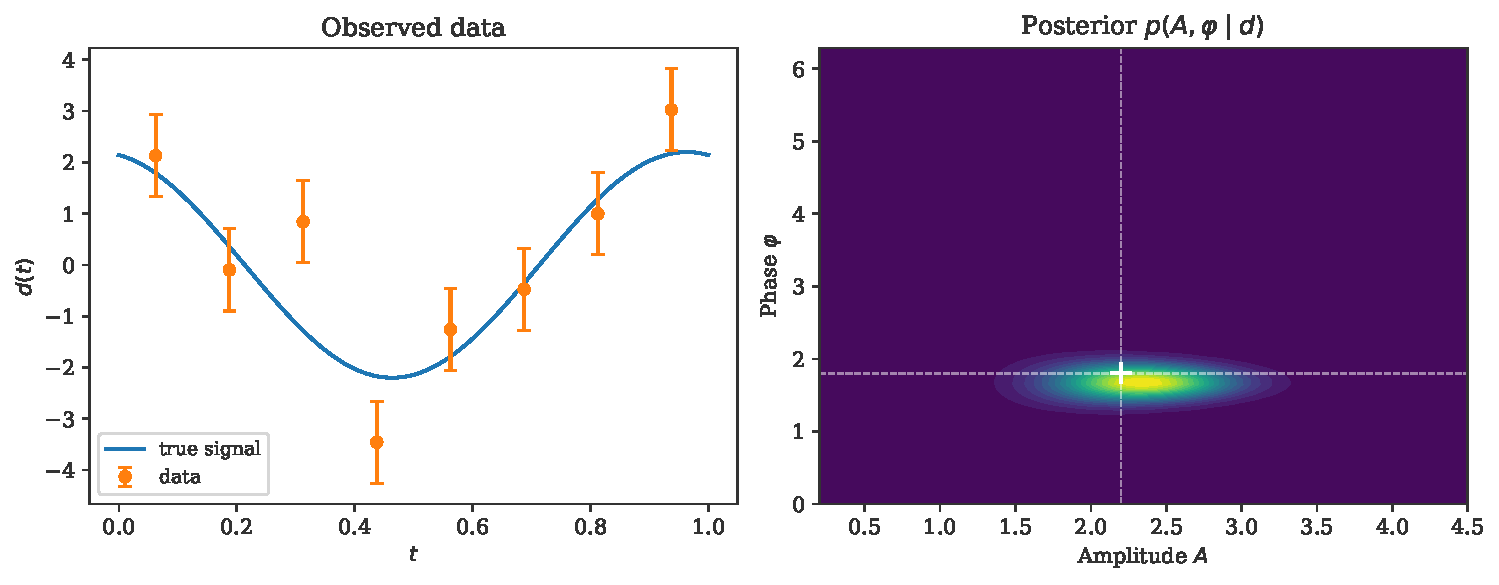
\includegraphics[width=\textwidth]{figures/sec1_data_and_posterior.pdf}
  \caption{%
    \textbf{Left:} Simulated data (orange) from the signal model
    Eq.~\eqref{eq:signal} with true parameters $A=2.2$, $\varphi=1.8$,
    $\sigma=0.8$, and $N=8$ observations.
    \textbf{Right:} The exact posterior $p(A, \varphi \mid d)$
    from Eq.~\eqref{eq:posterior}, showing
    the curved degeneracy ridge.
    White crosshairs mark the true values.
  }
  \label{fig:data-posterior}
\end{figure}

MCMC handles this, but at a cost.
A Metropolis--Hastings chain with isotropic proposals spends most
of its time proposing steps \emph{perpendicular} to the ridge, which
get rejected.
The result: highly correlated samples and an effective sample size
(ESS) much smaller than the chain length.

Can we do better?
What if, instead of walking through the posterior one step at a time,
we could learn a function that \emph{maps} a simple distribution directly
onto the posterior---and then generate as many independent samples as we
want?


%======================================================================
\section{The core idea: change of variables}
\label{sec:change-of-variables}
%======================================================================

The idea starts from something you already know: the
\emph{change-of-variables formula} from multivariate calculus.
Recall that if you have a random variable $z$ with known density
$q_0(z)$ and you apply a smooth, invertible transformation to get a new
variable $x$, you can write down the density of $x$ exactly---you just
need to account for how the transformation stretches or compresses
volume.

Let us set up the notation carefully, since several densities will be
in play.
We write $q_0$ for the \textbf{base density}---the simple distribution
we start from (a standard Gaussian $\mathcal{N}(0,I)$ in everything
that follows).
We write $f_\theta$ for a parametric, invertible, differentiable map
that we will learn; the subscript $\theta$ denotes the trainable
parameters.
Finally, $q_\theta$ denotes the \textbf{pushforward density}---the
distribution of $x = f_\theta(z)$ when $z \sim q_0$.
Note that $q_0$ and $q_\theta$ are \emph{different densities}: $q_0$
lives in the ``base'' space and $q_\theta$ lives in the ``target''
space; they are related by the transformation $f_\theta$, not by
a change of subscript.

With this notation, the change-of-variables formula gives us:
\begin{equation}
  q_\theta(x) = q_0\!\bigl(f_\theta^{-1}(x)\bigr)
  \left|\det \frac{\partial f_\theta^{-1}}{\partial x}\right|
  = q_0(z) \left|\det \frac{\partial f_\theta}{\partial z}\right|^{-1}.
  \label{eq:change-of-variables}
\end{equation}
The Jacobian matrix $\partial f_\theta / \partial z$ describes how
$f_\theta$ locally stretches each direction;
its determinant gives the overall volume change, and the absolute value
ensures the density stays non-negative.
If you have seen Jacobians in the context of coordinate transformations
in GR or in changing integration variables for a partition function,
this is exactly the same idea.

Now for the key insight.
Suppose we can find $\theta$ such that the pushforward $q_\theta$
matches the posterior $p$ we want to sample from.
Then sampling becomes trivial:
\begin{enumerate}[label=\arabic*.]
  \item Choose a parametric family of invertible maps $f_\theta$.
  \item Adjust $\theta$ until $q_\theta(x) \approx p(x \mid d)$.
  \item Sample: draw $z \sim \mathcal{N}(0, I)$,
        compute $x = f_\theta(z)$, done.
\end{enumerate}
Every sample is \emph{independent} (no chain, no burn-in, no thinning),
and the cost of generating each sample is just one forward pass through
$f_\theta$.
This is the essence of a \textbf{normalizing flow}.
The name ``normalizing'' refers to the fact that
Eq.~\eqref{eq:change-of-variables} keeps the density properly
normalized at every step; ``flow'' evokes the smooth, continuous
deformation of the base distribution into the target.


%======================================================================
\section{Planar flows: the simplest architecture}
\label{sec:planar}
%======================================================================

The simplest invertible layer is the \textbf{planar flow}
\cite{rezende2015}:
\begin{equation}
  f(z) = z + u\,\tanh(w^\top z + b),
  \label{eq:planar}
\end{equation}
where $u, w \in \mathbb{R}^2$ and $b \in \mathbb{R}$ are learnable
parameters---just \emph{five numbers} per layer.
This adds a $\tanh$ ``bump'' in the direction $u$, with the bump's
location and orientation controlled by $w$ and $b$.

The Jacobian determinant has a closed-form expression:
\begin{equation}
  \left|\det \frac{\partial f}{\partial z}\right|
  = \bigl|1 + u^\top \operatorname{diag}\!\bigl(1 - \tanh^2(w^\top z + b)\bigr)\,w\bigr|,
  \label{eq:planar-det}
\end{equation}
which is a scalar---trivially cheap to compute.

One layer can only perform a single directional warp---the bump is
always along $u$, so a single planar layer cannot, for instance,
simultaneously stretch in one direction and compress in another.
This is a real limitation: you need \emph{many} layers even
for modest 2D targets, and the directions $u_k$ of different layers
need not be orthogonal or evenly spread (they are learned, not
prescribed).
We will see in Section~\ref{sec:architectures} that more flexible
layer designs largely remove this bottleneck.

To build up expressiveness, we \textbf{compose} layers:
\begin{equation}
  f = f_K \circ f_{K-1} \circ \cdots \circ f_1.
  \label{eq:composition}
\end{equation}
The log-determinant of the composition is the sum of the per-layer
log-determinants (by the chain rule for Jacobians).
More layers means more expressive power, at a linear cost in computation.
Figure~\ref{fig:layer-deformation} illustrates this progressive
deformation: a standard 2D Gaussian is passed through an increasing
number of planar layers, each warping the distribution along one
learned direction.

% ---- Figure: layer-by-layer deformation ----
\begin{figure}[H]
  \centering
  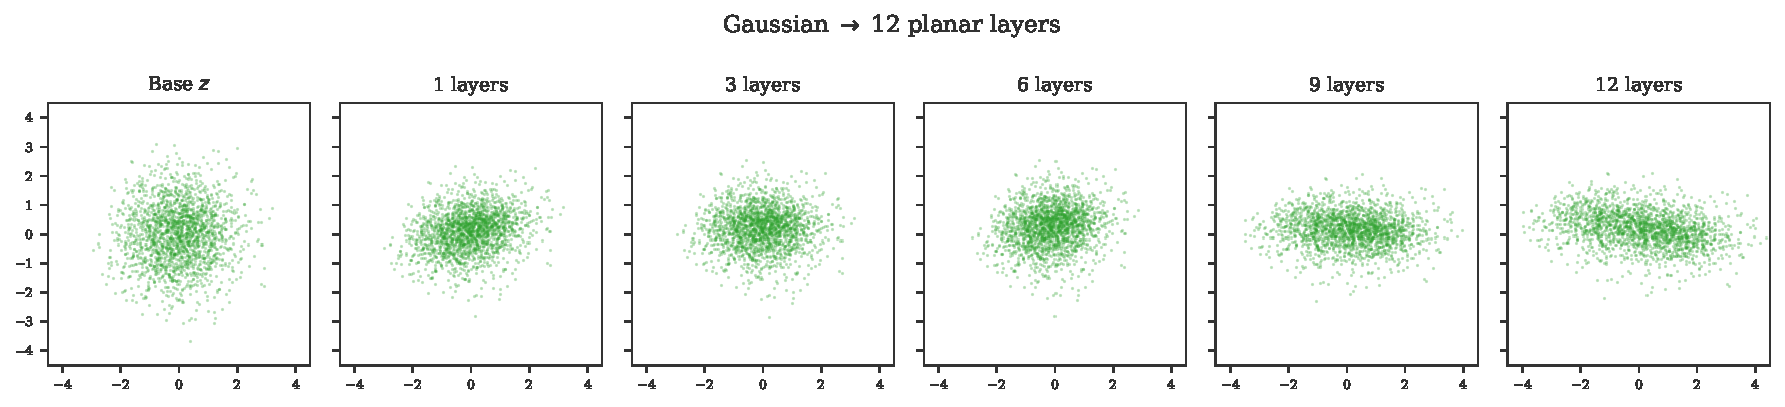
\includegraphics[width=\textwidth]{figures/sec3_layer_deformation.pdf}
  \caption{%
    A standard 2D Gaussian progressively deformed by planar flow
    layers (Eq.~\ref{eq:planar}), composed as in
    Eq.~\eqref{eq:composition}.
    Each layer warps the distribution along one learned direction.
    With enough layers, complex target geometries become accessible.
    The number of layers is adjustable via slider in the companion
    notebook.
  }
  \label{fig:layer-deformation}
\end{figure}


%======================================================================
\section{Training: minimizing KL divergence}
\label{sec:training}
%======================================================================

We want the flow's output distribution $q_\theta$ to match the target
posterior $p$.
We minimize the forward KL divergence:
\begin{equation}
  D_\mathrm{KL}(q_\theta \| p)
  = \mathbb{E}_{z \sim \mathcal{N}(0,I)} \left[
    -\log p\!\bigl(f_\theta(z)\bigr)
    - \log\left|\det \frac{\partial f_\theta}{\partial z}\right|
  \right] + \text{const}.
  \label{eq:kl-loss}
\end{equation}

Every term is computable \emph{without samples from $p$}:
\begin{itemize}
  \item $z \sim \mathcal{N}(0, I)$: draw from the base Gaussian (trivial).
  \item $f_\theta(z)$: push $z$ through the flow (forward pass).
  \item $\log p(f_\theta(z))$: evaluate the \emph{unnormalized} posterior
        at the output.
        The normalizing constant $p(d)$ is constant w.r.t.\ $\theta$ and
        drops out of the gradient.
  \item $\log|\det J|$: the flow architecture gives us this cheaply
        \emph{for the layer types we use here}.
        Planar flows have a rank-one update whose determinant is a
        scalar (Eq.~\ref{eq:planar-det}); affine coupling layers
        have a triangular Jacobian whose determinant is a product of
        diagonal entries (Section~\ref{sec:architectures}).
        This is \textbf{not free in general}---a na\"ive $d \times d$
        determinant costs $O(d^3)$, and much of the art in designing
        flow architectures is choosing transformations whose Jacobian
        structure makes the determinant cheap (triangular, rank-one, etc.).
\end{itemize}
There is \textbf{no training data} in the usual ML sense.
We are not fitting to examples; we are optimizing the flow parameters
so that its pushforward distribution matches a target that we can
evaluate pointwise.

\paragraph{The sigmoid transform.}
Since our physical parameters live on a bounded domain
(e.g., $A \in [0.2, 4.5]$), we map the flow's unbounded output through
a sigmoid:
$\theta_i = a_i + (b_i - a_i)\,\sigma(x_i)$.
This introduces an additional Jacobian factor $\log|J_\sigma|$ in
the loss.

\paragraph{Note on the KL direction (and how it can bite you).}
$D_\mathrm{KL}(q \| p)$ is \emph{mode-seeking}: it penalizes the flow
heavily for placing mass where $p$ is small (because $\log(q/p)$ blows
up), but imposes \emph{no direct penalty} for regions where $p$ has
mass but $q$ does not.
The practical consequence is that if the target has multiple modes, the
flow may latch onto one mode and ignore the others entirely.
For a bimodal posterior, this means you could obtain a perfectly
converged-looking loss curve and a set of samples that appear
self-consistent---yet miss half the posterior.
There is nothing in the training signal that tells you a mode was
missed; you only discover the problem by independent validation
(e.g., a short MCMC run, a p--p plot, or physical intuition about
the expected degeneracies).

The reverse direction, $D_\mathrm{KL}(p \| q)$, would be
\emph{mode-covering}: it forces $q$ to have support everywhere $p$ does.
But it requires samples from $p$---which is what we are trying to
obtain in the first place.
In practice, one can partially mitigate the mode-seeking problem by
using the flow as a proposal for MCMC (Section~\ref{sec:open}), or
by training with alternative divergences ($\alpha$-divergences,
the sliced Wasserstein distance) that interpolate between the two
extremes.
This asymmetry matters most for multimodal targets
(Section~\ref{sec:architectures}), and is one of the main open
challenges in applying normalizing flows to problems with well-separated
modes---such as the sky-localization degeneracy in GW inference.

Figure~\ref{fig:training} shows this training procedure applied to our
sinusoidal posterior: the KL loss (Eq.~\ref{eq:kl-loss}) decreases
over 800 epochs, and the trained flow produces samples that closely
match the exact posterior.

% ---- Figure: training convergence ----
\begin{figure}[H]
  \centering
  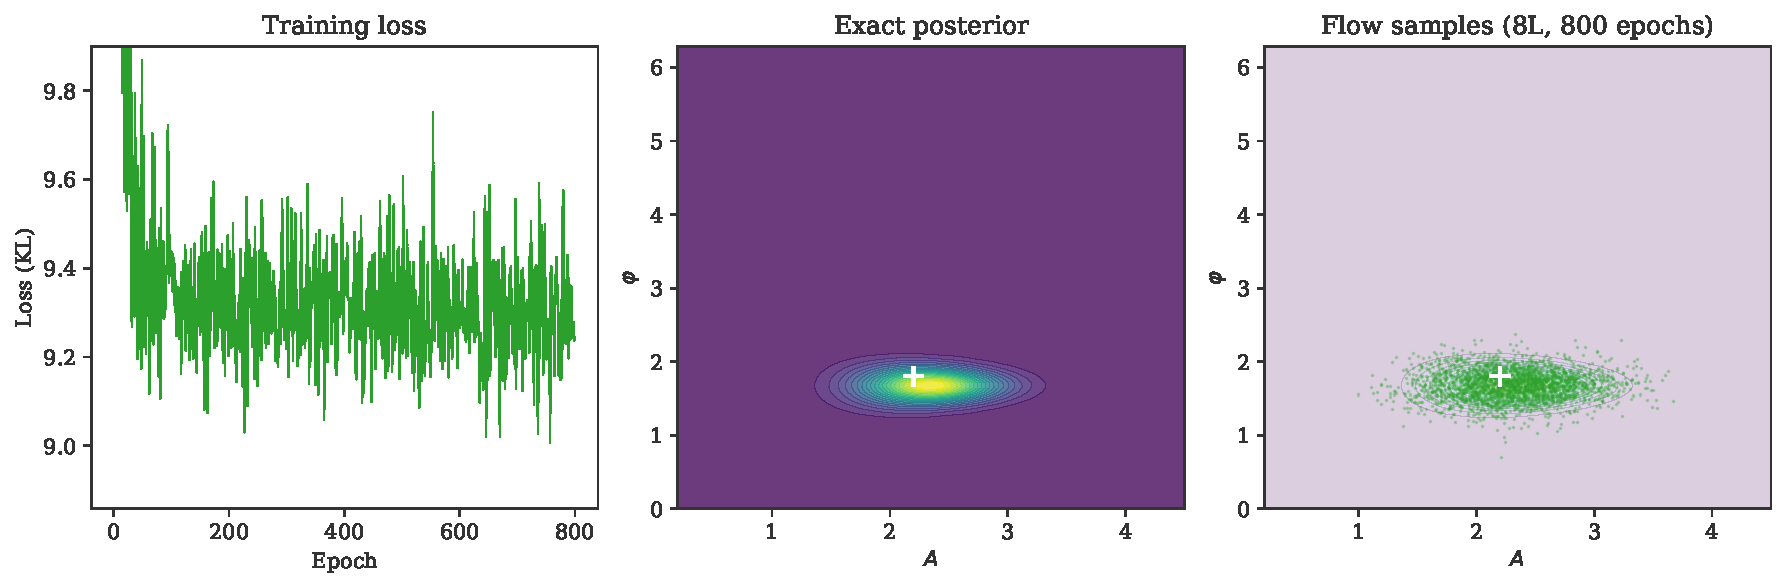
\includegraphics[width=\textwidth]{figures/sec4_training.pdf}
  \caption{%
    Training a planar flow on the sinusoidal posterior
    (Eq.~\ref{eq:posterior}) by minimizing the KL divergence
    (Eq.~\ref{eq:kl-loss}).
    \textbf{Left:} Loss vs.\ epoch, showing convergence.
    \textbf{Center:} Exact posterior.
    \textbf{Right:} Samples from the trained flow (8 layers, 800 epochs).
  }
  \label{fig:training}
\end{figure}


%======================================================================
\section{MCMC vs.\ normalizing flows: head to head}
\label{sec:comparison}
%======================================================================

The fundamental difference between MCMC and normalizing flows lies
in \emph{where the computational cost is paid}.

\paragraph{MCMC (Metropolis--Hastings).}
Cost is at inference time.
Each step proposes a move, evaluates $p$, and accepts or rejects.
Samples are correlated, so the effective sample size satisfies
$\mathrm{ESS} \ll N$ for a chain of length $N$.
The ESS is computed from the autocorrelation function:
\begin{equation}
  \mathrm{ESS} = \frac{N}{1 + 2\sum_{k=1}^{K} \hat{\rho}(k)},
  \label{eq:ess}
\end{equation}
where $\hat{\rho}(k)$ is the estimated autocorrelation at lag $k$,
truncated when $\hat{\rho}(k) < 0.05$.

\paragraph{Normalizing flow.}
Cost is upfront during training.
Once trained, sampling is nearly free: draw $z \sim \mathcal{N}(0, I)$,
push through $f_\theta$, and obtain an independent posterior sample.
$\mathrm{ESS} = N$ by construction.
However, the training cost itself depends strongly on the architecture:
a simple planar flow with 5 parameters per layer trains in seconds,
while a production neural spline flow with deep ResNet conditioners can
require hours of GPU time.
For a one-off inference on a single event, this upfront cost may exceed
the cost of running MCMC; the payoff comes when the trained flow is
reused (amortized inference) or when many independent samples are
needed quickly.

Table~\ref{tab:comparison} summarizes the tradeoffs, and
Figure~\ref{fig:mcmc-vs-flow} compares the two methods side by side
on the sinusoidal posterior from Section~\ref{sec:problem}.

\begin{table}[ht]
  \centering
  \caption{MCMC vs.\ normalizing flow comparison.}
  \label{tab:comparison}
  \begin{tabular}{lll}
    \toprule
    & \textbf{MCMC} & \textbf{Normalizing Flow} \\
    \midrule
    Cost location     & Inference time (per sample) & Training time (upfront) \\
    Sample independence & Correlated (ESS $\ll N$) & Independent (ESS $= N$) \\
    Burn-in           & Required & None \\
    Exactness         & Asymptotically exact & Approximate (finite capacity) \\
    Architecture choices & Proposal tuning only & Layer type, depth, width \\
    Parallelism       & Sequential chain & Fully parallelizable \\
    Amortization      & None & Reusable across datasets$^*$ \\
    \bottomrule
    \multicolumn{3}{l}{\small $^*$With simulation-based training (Section~\ref{sec:gw}).}
  \end{tabular}
\end{table}

% ---- Figure: MCMC vs flow ----
\begin{figure}[H]
  \centering
  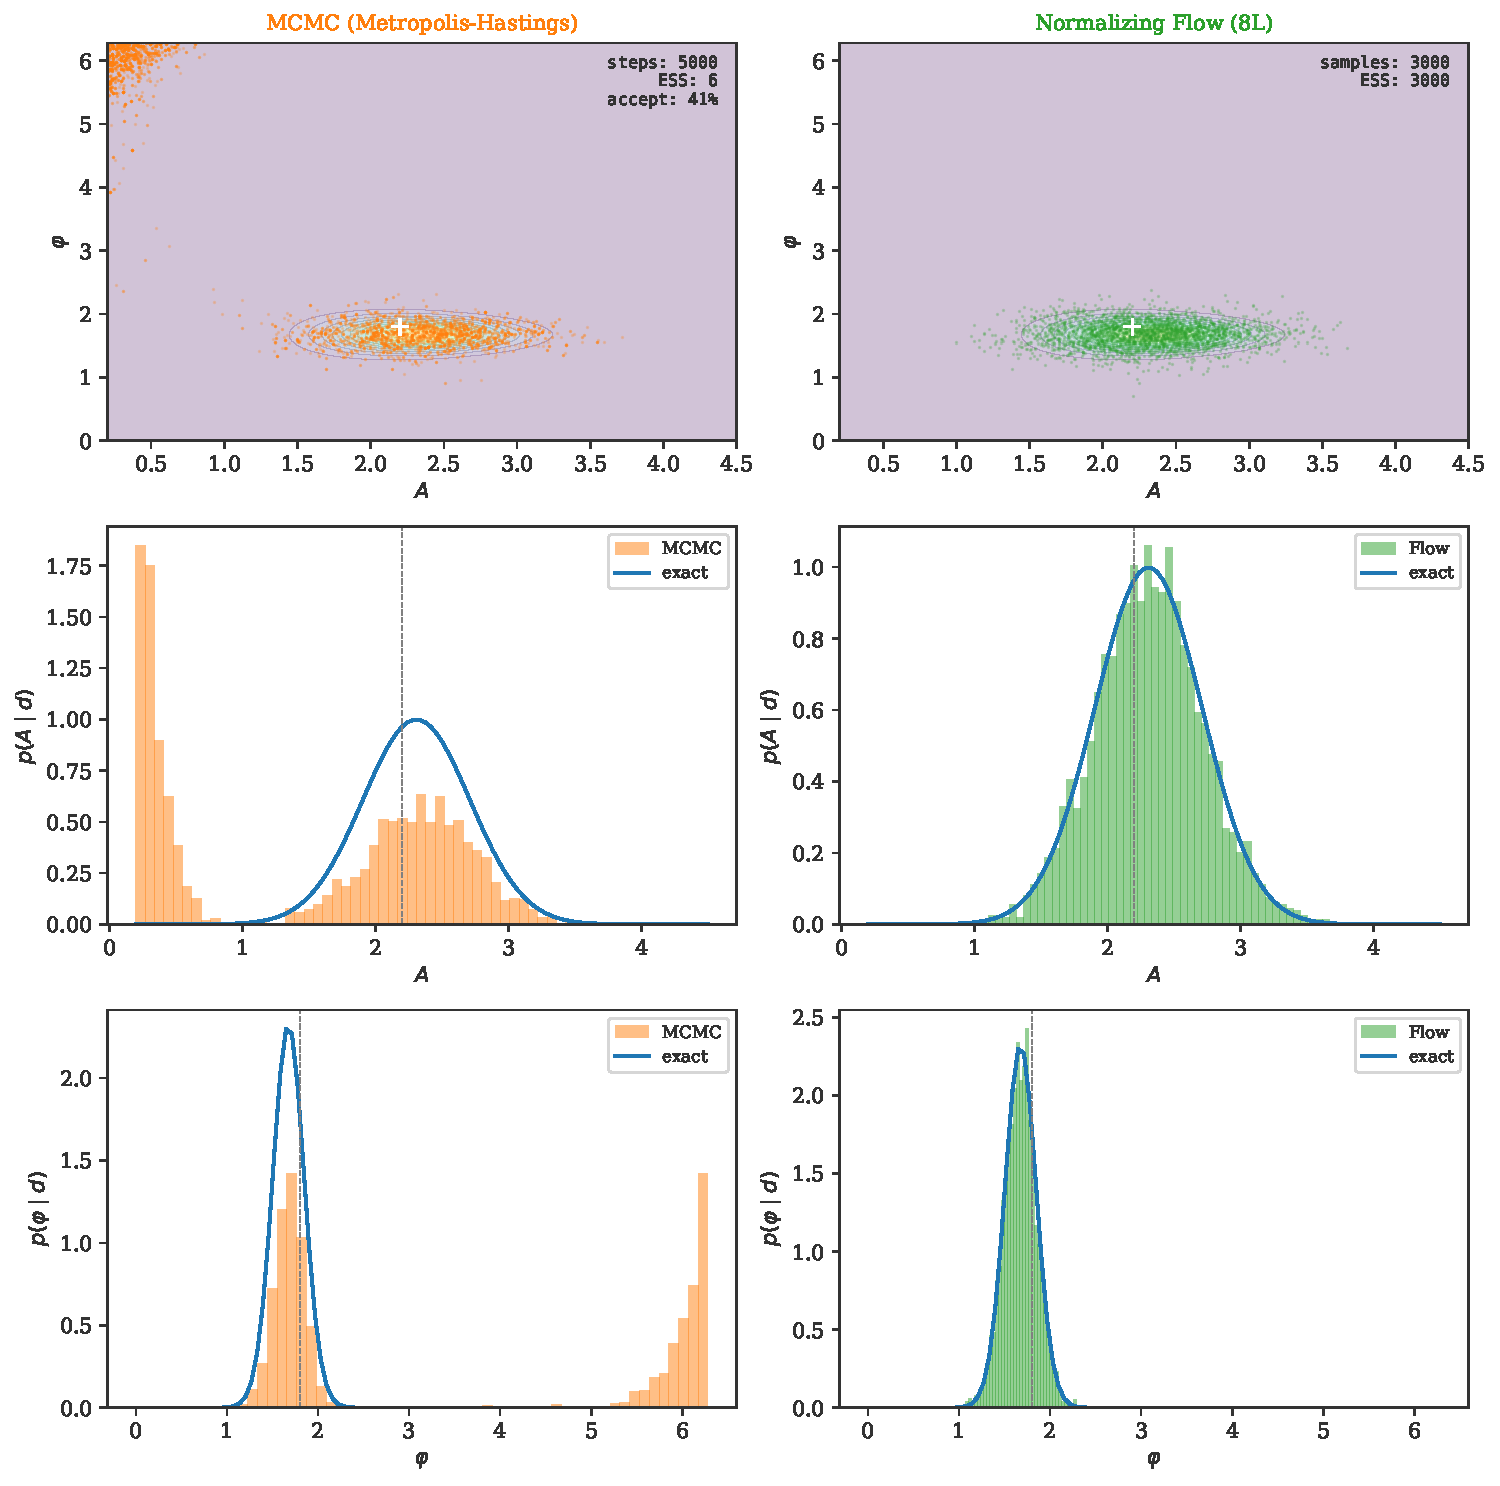
\includegraphics[width=\textwidth]{figures/sec5_mcmc_vs_flow.pdf}
  \caption{%
    Head-to-head comparison on the sinusoidal posterior
    (Eq.~\ref{eq:posterior}).
    \textbf{Left column:} MCMC (Metropolis--Hastings, 5000 steps);
    the effective sample size (Eq.~\ref{eq:ess}) is much smaller than
    the chain length.
    \textbf{Right column:} Normalizing flow (8 planar layers,
    800 epochs); every sample is independent, so ESS~$= N$.
    Top row: 2D scatter overlaid on the exact posterior.
    Middle and bottom rows: marginal posteriors for $A$ and $\varphi$
    compared to the exact solution (blue curves).
  }
  \label{fig:mcmc-vs-flow}
\end{figure}


%======================================================================
\section{Architecture matters}
\label{sec:architectures}
%======================================================================

Planar flows are pedagogically useful but limited.
Here we compare three architectures, all using the same number of
layers and the same training procedure.
Figure~\ref{fig:grid-deformation} visualizes how a single layer of
each architecture deforms a regular grid, providing geometric intuition
for the equations that follow.

\subsection{Planar flow}
As defined in Eq.~\eqref{eq:planar}: 5 parameters per layer.
Each layer can only warp along one direction defined by $w$.

\subsection{Radial flow}
\begin{equation}
  f(z) = z + \beta\,h(\alpha, r)\,(z - z_0),
  \qquad h(\alpha, r) = \frac{1}{\alpha + r},
  \qquad r = \|z - z_0\|,
  \label{eq:radial}
\end{equation}
with 4 parameters per layer ($z_0 \in \mathbb{R}^2$, $\alpha > 0$, $\beta$).
This expands or contracts space radially around a learned center $z_0$.
Good for changing the spread of a distribution, but cannot introduce
correlations between dimensions.

The Jacobian determinant in $d$ dimensions is:
\begin{equation}
  \det J = (1 + \beta h)^{d-1}\,(1 + \beta h + \beta h' r),
  \qquad h' = -h^2.
\end{equation}

\subsection{Affine coupling (RealNVP-style)}
This architecture was introduced by Dinh et~al.\ \cite{dinh2017} under
the name \textbf{RealNVP} (``Real-valued Non-Volume Preserving
transformations''), building on the earlier NICE framework
\cite{dinh2014} which used additive (volume-preserving) coupling layers.
The key idea is to split the input dimensions into two groups: one group
passes through unchanged and serves as the input to a \emph{conditioner}
function that determines how the other group is transformed.
RealNVP's affine coupling was further extended by Glow
\cite{kingma2018}, which replaced fixed permutations with learned
invertible $1 \times 1$ convolutions.
Our implementation is a simplified 2D version of the RealNVP
architecture, using a single $\tanh$ unit as the conditioner instead
of a deep neural network.

Split the input as $z = (z_a, z_b)$.
One dimension passes through unchanged; the other receives a learned
scale and shift conditioned on the first:
\begin{equation}
  x_a = z_a, \qquad x_b = z_b \cdot e^{s(z_a)} + t(z_a),
  \label{eq:coupling}
\end{equation}
where $s$ and $t$ are parameterized functions of $z_a$.
In our implementation, $s(z_a) = a_1 \tanh(a_2 z_a + a_3) + a_4$
(and similarly for $t$), giving 8 parameters per layer.
Alternating which dimension is held fixed ensures both dimensions
are transformed.

The Jacobian is triangular, so its determinant is simply
$\exp\!\bigl(\sum_i s_i(z_a)\bigr)$---no matrix computation needed.

This is the simplified version of the architecture used in
DINGO and other production tools, where $s$ and $t$ are deep
neural networks with thousands of parameters.

% ---- Figure: grid deformation by architecture ----
\begin{figure}[H]
  \centering
  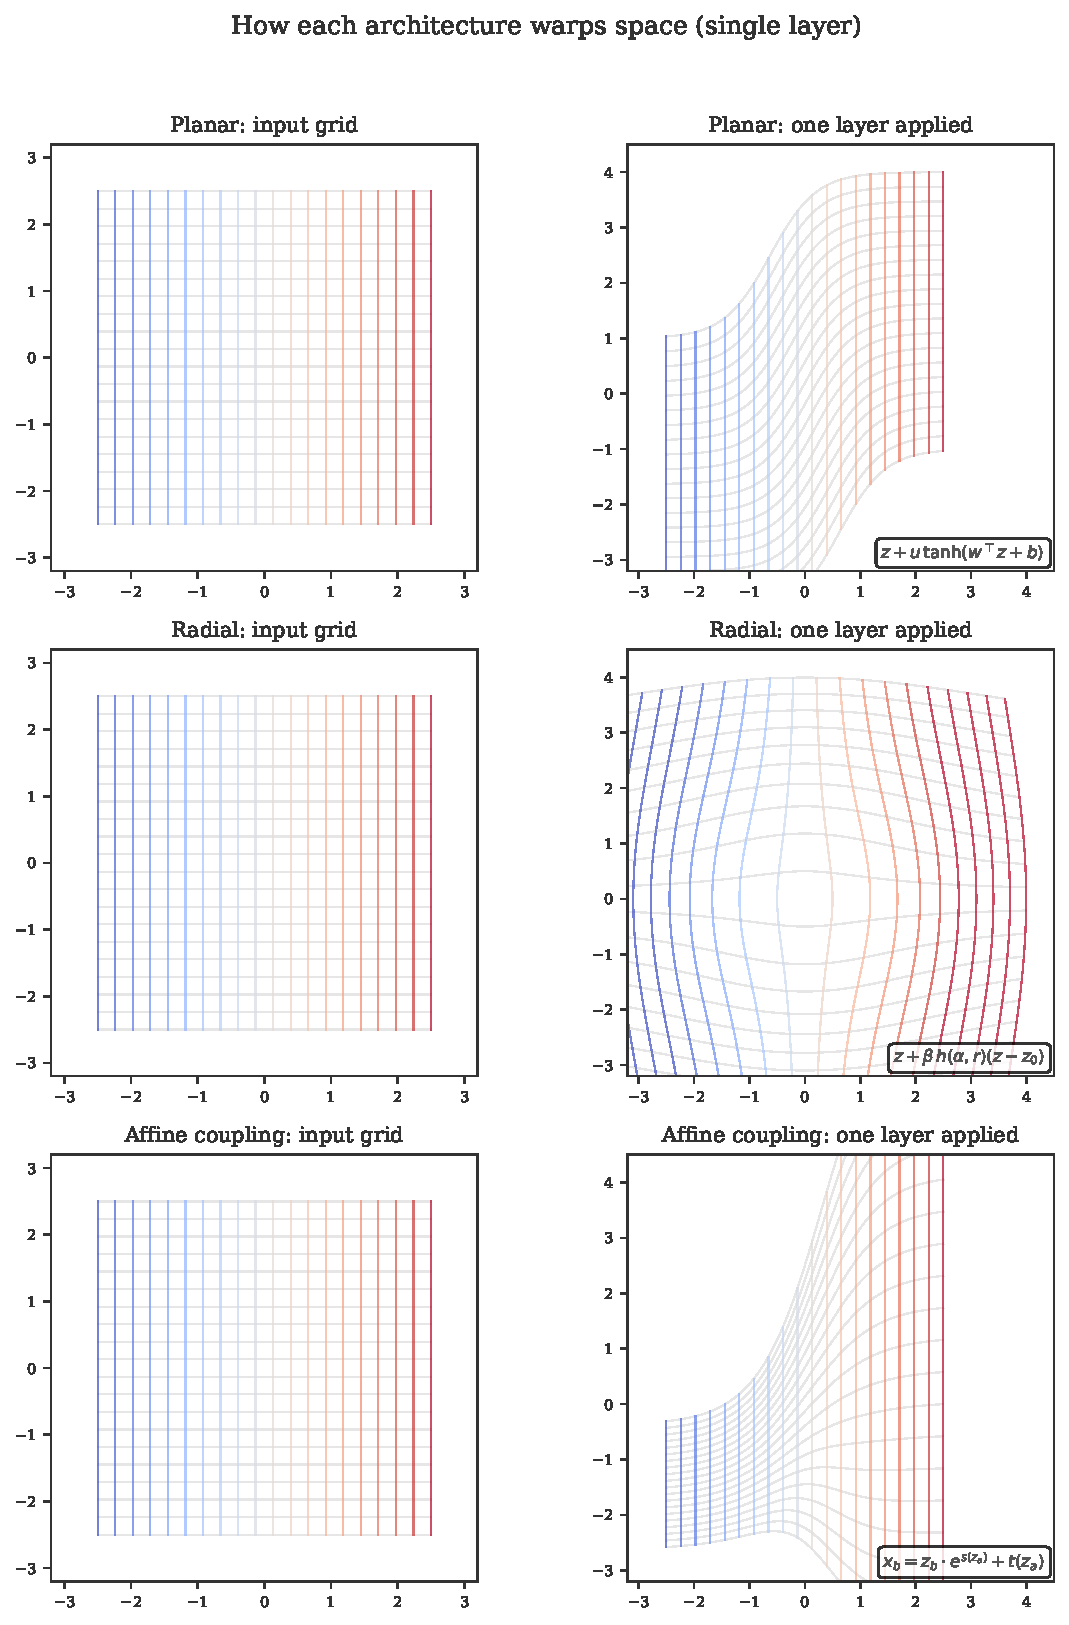
\includegraphics[width=\textwidth]{figures/sec6_grid_deformation.pdf}
  \caption{%
    How each architecture warps a regular grid.
    Columns show the input grid, the result after one layer, and the
    result after ten layers.
    \textbf{Planar} (top row): the $\tanh$ bump in
    Eq.~\eqref{eq:planar} displaces grid lines along
    the direction $u$, producing a directional shear near the hyperplane
    $w^\top z + b = 0$.
    \textbf{Radial} (middle row): the radial transform in
    Eq.~\eqref{eq:radial} expands or contracts space around
    the center $z_0$, preserving angular symmetry.
    \textbf{Affine coupling} (bottom row): the coupling layer in
    Eq.~\eqref{eq:coupling} holds one coordinate fixed while
    applying a conditional scale and shift to the other, producing an
    axis-aligned but nonlinear deformation.
    Grid lines are colored by original $x$-position to track how
    regions of space move.
  }
  \label{fig:grid-deformation}
\end{figure}

\subsection{Comparison across target distributions}

We test all three architectures on five target distributions of
increasing difficulty (Figure~\ref{fig:architectures} shows a
representative comparison):
\begin{enumerate}
  \item \textbf{Sinusoid}: curved ridge from amplitude--phase degeneracy.
  \item \textbf{Banana} (Rosenbrock): strong nonlinear correlation $y \approx x^2$.
  \item \textbf{Triple mode}: three overlapping Gaussians with different orientations.
  \item \textbf{Ring}: annular posterior at $r \approx 3$---a topological
        challenge since smooth diffeomorphisms cannot ``punch a hole''
        in a simply connected base distribution.
  \item \textbf{Funnel} (Neal): hierarchical pathology where the width
        in $x_1$ varies exponentially with $x_2$.
\end{enumerate}

% ---- Figure: architecture comparison ----
\begin{figure}[H]
  \centering
  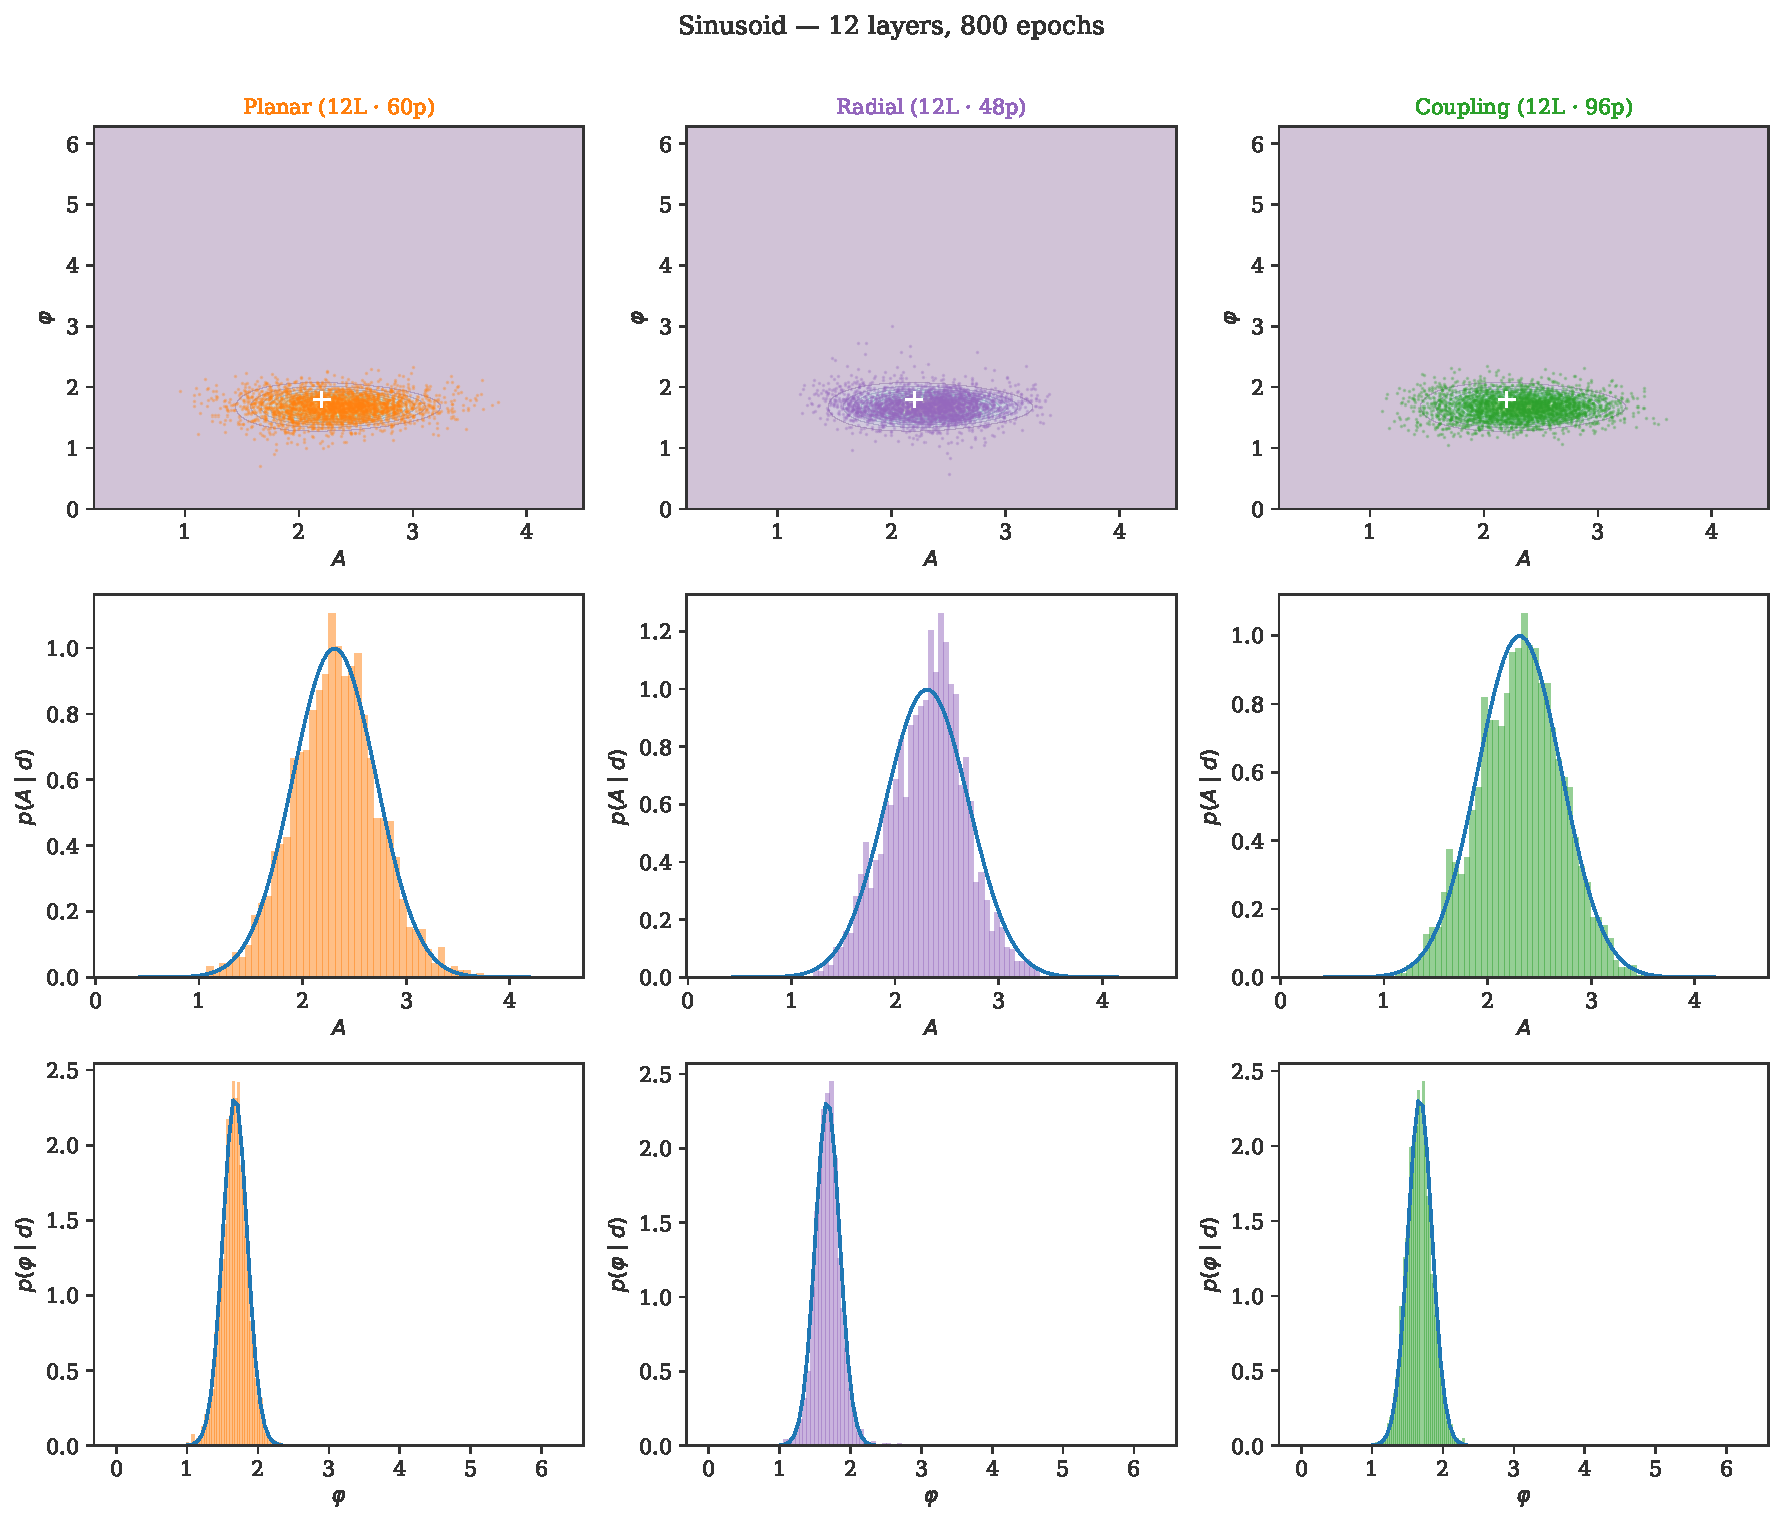
\includegraphics[width=\textwidth]{figures/sec6_architecture_comparison.pdf}
  \caption{%
    Architecture comparison on the sinusoidal posterior
    (Eq.~\ref{eq:posterior}), all trained with the KL objective
    (Eq.~\ref{eq:kl-loss}) for 800 epochs with 12 layers each.
    Columns from left to right: planar
    (Eq.~\ref{eq:planar}), radial (Eq.~\ref{eq:radial}),
    and affine coupling (Eq.~\ref{eq:coupling}).
    Top row: 2D samples overlaid on the exact posterior.
    Middle and bottom rows: marginal posteriors for $A$ and $\varphi$
    vs.\ exact (blue).
    The distribution, layer count, and epoch count are all adjustable
    in the companion notebook.
  }
  \label{fig:architectures}
\end{figure}

Table~\ref{tab:arch-summary} summarizes which architecture performs
best on each target.
The companion notebook lets you verify these observations
interactively by selecting different distributions from the dropdown
and comparing the results.

\begin{table}[H]
  \centering
  \caption{Architecture performance across target distributions.
    \cmark\ = captures the target well;
    $\sim$ = partial success;
    \xmark\ = fails qualitatively.}
  \label{tab:arch-summary}
  \begin{tabular}{lccc}
    \toprule
    \textbf{Target} & \textbf{Planar} & \textbf{Radial} & \textbf{Coupling} \\
    \midrule
    Sinusoid & $\sim$ & $\sim$ & \cmark \\
    Banana   & $\sim$ & \xmark & \cmark \\
    Triple mode & \xmark & \xmark & $\sim$ \\
    Ring     & \xmark & \xmark & $\sim$ \\
    Funnel   & \xmark & \xmark & $\sim$ \\
    \bottomrule
  \end{tabular}
\end{table}

Key observations:
\begin{itemize}
  \item \textbf{Sinusoid}: All three produce reasonable samples;
        the coupling flow captures the curved ridge most faithfully
        because its conditional scale parameter can model the
        $A$-dependent width of the ridge in $\varphi$.
  \item \textbf{Banana}: The coupling flow wins decisively---its
        scale function $s(z_a)$ directly models the $x$-dependent
        variance $\mathrm{Var}(y \mid x) \propto 1$.
        Radial flows cannot introduce correlations between dimensions
        at all and collapse to a blob.
  \item \textbf{Triple mode}: All architectures struggle because of
        the mode-seeking KL (Section~\ref{sec:training}): the flow
        typically locks onto one or two modes and ignores the rest.
        Coupling flows fare best because their per-layer expressiveness
        is highest, but even they rarely cover all three modes.
        This is the mode-seeking problem in action.
  \item \textbf{Ring}: None of the architectures can fully evacuate
        the interior, since all three are smooth diffeomorphisms
        and therefore preserve the topology of the (simply connected)
        base distribution.
        Planar flows produce spirals; coupling flows approximate the
        ring more closely by squeezing the interior mass into a thin
        annulus.
  \item \textbf{Funnel}: The exponential variation in width is hard
        for all methods.
        Coupling flows have the best chance because their scale
        parameter directly models the changing conditional width, but
        even they require many layers.
\end{itemize}


%======================================================================
\section{From toy models to gravitational-wave inference}
\label{sec:gw}
%======================================================================

Everything in this tutorial uses 2D posteriors with 5--8 parameters
per layer and finite-difference gradients.
Real applications differ in scale but not in principle.

\paragraph{DINGO} \cite{dax2021} uses normalizing flows for compact
binary coalescence (CBC) parameter estimation---15+ dimensional
posteriors with coupling layers whose conditioners are deep residual
networks (thousands of parameters per layer), trained with automatic
differentiation on GPUs.
A \emph{conditioner} is the function inside a coupling layer that
computes the transformation parameters from the untransformed
variables---in our toy model this is a simple $\tanh$ function
(Eq.~\ref{eq:coupling}), but in DINGO it is a deep
\emph{residual network} (ResNet), a neural network architecture in
which each layer adds a learned residual to its input
($\mathrm{output} = x + F(x)$), making it possible to train very deep
networks without degradation.
Note that DINGO uses a \textbf{discrete} flow (a finite composition of
coupling layers), not a continuous normalizing flow
(Section~\ref{sec:open}).
The use of automatic differentiation (AD) for computing parameter
gradients during \emph{training} does not make the flow itself
continuous---AD replaces our finite-difference gradient hack with exact
backpropagation, but the learned map $f_\theta$ is still a fixed
sequence of discrete layers.
Crucially, DINGO uses \emph{simulation-based inference}: it trains on
simulated pairs $(\theta_i, d_i) \sim p(\theta)\,p(d|\theta)$ and
learns the conditional posterior $p(\theta | d)$ amortized over many
possible datasets.
This means a single trained network can produce posteriors for new
events in seconds, without retraining.

\paragraph{Overlapping signals.}
Third-generation detectors (Einstein Telescope, Cosmic Explorer) will
have detection rates high enough that CBC signals routinely overlap in
time.
Joint parameter estimation of overlapping events is preferable to
hierarchical analysis but is computationally demanding with traditional
samplers.
Langendorff et~al.\ \cite{langendorff2023} demonstrated a
proof-of-concept using \emph{conditional continuous normalizing flows}
for this problem.
The key ideas: (i)~the flow is \emph{conditional}---the transformation
$f_\theta(z; d)$ depends on the observed data $d$, so a single trained
network produces posteriors for different datasets without retraining
(as in DINGO); (ii)~the flow is \emph{continuous}---rather than a
fixed sequence of discrete coupling layers, the transformation is
defined by a neural ODE (Section~\ref{sec:open}), with the velocity
field parameterized by a hypernetwork whose external inputs smoothly
modulate the dynamics.
The continuous formulation keeps the memory footprint small (no need to
store activations at every discrete layer for backpropagation), and
the conditional structure means the 3D Gaussian base is mapped to the
complex joint posterior of overlapping events by minimizing the KL
divergence.
Results show slightly widened posteriors compared to full MCMC, but
injected values are always recovered, and inference is orders of
magnitude faster after training.

\paragraph{Population inference.}
Cheung et~al.\ \cite{cheung2022} tested normalizing flows as
likelihood emulators for GW population inference, finding that flows
successfully recover population posteriors using up to 300 mock
injections where Gaussian process regression fails in high dimensions.
The caveat: flows can underestimate uncertainty on real data, so
validation against traditional methods remains essential.

\paragraph{nessai} \cite{williams2021} combines normalizing flows with
nested sampling, using the flow as a proposal distribution to
accelerate evidence computation.

\paragraph{Architectural upgrades.}
The key difference from our toy implementation is in the
\emph{conditioner}---the function inside a coupling layer that computes
the scale and shift from the untransformed variables (see Glossary).
Our coupling layers use $s(z_a) = a_1 \tanh(a_2 z_a + a_3) + a_4$
(4~parameters).
Production flows replace this with $s(z_a) = \mathrm{ResNet}(z_a)$,
a residual network (see Glossary) with tens of thousands of parameters,
or \emph{neural spline flows} \cite{durkan2019} where the
transformation is a monotonic rational-quadratic spline, providing
much greater flexibility per layer.
An alternative to coupling layers are \emph{autoregressive} flows
\cite{kingma2016,papamakarios2017}, which condition each dimension on
all preceding dimensions rather than on a fixed partition; these are
more expressive per layer but slower to sample from.

Automatic differentiation (via PyTorch or JAX) replaces our
finite-difference gradients, giving exact gradients at comparable cost.
GPU parallelism enables batch sizes in the thousands and training on
millions of simulated waveforms.


%======================================================================
\section{Open questions}
\label{sec:open}
%======================================================================

\paragraph{Mode coverage vs.\ mode seeking.}
Training with $D_\mathrm{KL}(q \| p)$ is mode-seeking; the flow
may nail one or two modes while missing others.
Alternative objectives include the reverse KL (requires target
samples), $\alpha$-divergences, and the sliced Wasserstein distance.
In practice, mode coverage is validated with p--p plots and
comparison against short MCMC runs.

\paragraph{Combining flows with MCMC.}
Use the trained flow as a proposal distribution for
Metropolis--Hastings or Hamiltonian Monte Carlo.
The flow provides good proposals (high acceptance rate), while
MCMC guarantees asymptotic exactness---even if the flow is imperfect.
Concretely, one draws $z \sim \mathcal{N}(0,I)$, pushes through
$f_\theta$ to get a proposal $x' = f_\theta(z)$, and accepts or
rejects via the usual Metropolis ratio using the \emph{true} posterior
$p(x' \mid d)$.
Because the flow already approximates $p$, the acceptance rate is high
(often $> 80\%$), and the chain mixes rapidly even for strongly
correlated posteriors.
This also provides a self-consistency check: if the Metropolis chain
discovers regions of high posterior mass that the flow missed (i.e.,
modes dropped by the mode-seeking KL), the acceptance rate in those
regions will be low, flagging the problem.
The nessai package \cite{williams2021} implements a variant of this
idea with nested sampling rather than MCMC.
This combination is arguably the most practical near-term use of
normalizing flows in GW inference: you get the speed of a flow-based
proposal with the statistical guarantees of MCMC.

\paragraph{A taxonomy of flow architectures.}
This tutorial covers only three simple layer types.
The broader landscape, reviewed in \cite{kobyzev2021,papamakarios2021},
includes several important families:
\begin{itemize}
  \item \textbf{Elementwise flows}: apply a scalar bijection $h$ to
        each dimension independently.
        The Jacobian is diagonal ($\det J = \prod |h'(x_i)|$), so
        inversion and density evaluation are trivially cheap---but the
        transformation cannot capture correlations between dimensions.
  \item \textbf{Linear flows}: $g(x) = Ax + b$ with $A$ invertible.
        $\det J = \det A$, which is $O(d^3)$ for a full matrix.
        In practice, $A$ is restricted to be triangular, diagonal, or
        orthogonal to keep the cost manageable.
        Linear flows are not expressive on their own (a Gaussian stays
        Gaussian) but serve as building blocks---for example, the
        $1 \times 1$ convolutions in Glow \cite{kingma2018} are learned
        linear layers that replace fixed permutations.
  \item \textbf{Autoregressive flows}
        \cite{kingma2016,papamakarios2017}: generalize triangular linear
        maps by conditioning each dimension on all preceding ones.
        The Jacobian is triangular, so $\det J$ is a product of diagonal
        entries.
        More expressive per layer than coupling flows, but sampling
        requires a sequential pass through dimensions (cannot be
        parallelized).
        Inverse autoregressive flows (IAF) reverse the direction:
        fast to sample from, slow for density evaluation.
  \item \textbf{Residual flows}: $g(x) = x + F(x)$ where $F$ is a
        neural network with a Lipschitz constraint to ensure
        invertibility.
        The Jacobian determinant requires a power-series estimator,
        making it more expensive than coupling or autoregressive flows.
  \item \textbf{Continuous normalizing flows}: replace discrete layers
        with a neural ODE \cite{chen2018}:
        \begin{equation}
          \frac{dx}{dt} = v_\theta(x, t),
        \end{equation}
        where the log-density evolves as
        $\frac{\partial \log q}{\partial t} = -\nabla \cdot v$
        (the instantaneous change-of-variables formula).
        FFJORD \cite{grathwohl2018} made this practical by replacing the
        exact trace with a stochastic Hutchinson estimator.
        This removes the need to choose a fixed number of layers, at the
        cost of solving an ODE during training and sampling.
        This is the architecture used by Langendorff et~al.\
        \cite{langendorff2023} for overlapping GW signals
        (Section~\ref{sec:gw}).
\end{itemize}
Each family makes a different tradeoff between expressiveness,
inversion cost, and Jacobian computation cost.
The choice of architecture imposes an inductive bias on the class of
distributions the flow can represent efficiently, and which architecture
is best depends on whether the application requires fast sampling, fast
density evaluation, or both.

\paragraph{Simulation-based inference (SBI).}
When the likelihood $p(d|\theta)$ is intractable (you can simulate but
cannot write it down), flows can be trained on simulated pairs
$(\theta, d)$ to learn the conditional posterior amortized over many
datasets.
This is the approach used by DINGO for gravitational-wave parameter
estimation, and is increasingly adopted across physics.

\paragraph{Further open problems.}
Several questions remain active areas of research:
the role of the base distribution (usually Gaussian, but other choices
may provide better inductive biases for specific problems);
the choice of loss function (alternatives to KL divergence may be
better suited for certain target geometries);
flows on non-Euclidean manifolds (relevant when parameters live on
spheres, tori, or other constrained spaces---e.g., sky location in
GW inference);
and flows for discrete distributions, which require fundamentally
different approaches since smooth bijections are inherently continuous.


%======================================================================
\section*{Running the interactive tutorial}
%======================================================================

The companion notebook (\texttt{tutorial.py}) is a
\href{https://marimo.io}{marimo} reactive notebook.
To run it:
\begin{lstlisting}[language=bash]
pip install -r requirements.txt
marimo edit tutorial.py
\end{lstlisting}

All figures in this document can be regenerated from the notebook.
The recommended workflow:
\begin{enumerate}
  \item Run the notebook with default slider values.
  \item Export each figure cell as PDF using matplotlib's
        \texttt{savefig}.
  \item Place the exported figures in the \texttt{figures/} directory.
\end{enumerate}

A helper script for batch export is provided in
\texttt{export\_figures.py} (if generated).

\vspace{1em}
\noindent\rule{\textwidth}{0.4pt}
\vspace{0.5em}
\noindent\textit{Tutorial by Chiara Mingarelli, Abigail Moran, and
Nicole Khusid (Yale University / Flatiron Institute CCA), 2026.}


%======================================================================
% References
%======================================================================
\begin{thebibliography}{9}

\bibitem{rezende2015}
D.~J. Rezende and S.~Mohamed,
``Variational inference with normalizing flows,''
\textit{Proceedings of the 32nd International Conference on Machine Learning (ICML)}, 2015.
\href{https://arxiv.org/abs/1505.05770}{arXiv:1505.05770}.

\bibitem{dax2021}
M.~Dax, S.~R. Green, J.~Gair, J.~H. Macke, A.~Buonanno, and B.~Sch\"olkopf,
``Real-time gravitational wave science with neural posterior estimation,''
\textit{Physical Review Letters}, \textbf{127}(24):241103, 2021.
\href{https://arxiv.org/abs/2106.12594}{arXiv:2106.12594}.

\bibitem{williams2021}
M.~J. Williams, J.~Veitch, and C.~Messenger,
``Nested sampling with normalizing flows for gravitational-wave inference,''
\textit{Physical Review D}, \textbf{103}(10):103006, 2021.
\href{https://arxiv.org/abs/2102.11056}{arXiv:2102.11056}.

\bibitem{dinh2017}
L.~Dinh, J.~Sohl-Dickstein, and S.~Bengio,
``Density estimation using Real-NVP,''
\textit{International Conference on Learning Representations (ICLR)}, 2017.
\href{https://arxiv.org/abs/1605.08803}{arXiv:1605.08803}.

\bibitem{papamakarios2021}
G.~Papamakarios, E.~Nalisnick, D.~J. Rezende, S.~Mohamed, and B.~Lakshminarayanan,
``Normalizing flows for probabilistic modeling and inference,''
\textit{Journal of Machine Learning Research}, \textbf{22}(57):1--64, 2021.
\href{https://arxiv.org/abs/1912.02762}{arXiv:1912.02762}.

\bibitem{kobyzev2021}
I.~Kobyzev, S.~J.~D. Prince, and M.~A. Brubaker,
``Normalizing flows: an introduction and review of current methods,''
\textit{IEEE Transactions on Pattern Analysis and Machine Intelligence},
\textbf{43}(11):3964--3979, 2021.

\bibitem{cranmer2020}
K.~Cranmer, J.~Brehmer, and G.~Louppe,
``The frontier of simulation-based inference,''
\textit{Proceedings of the National Academy of Sciences},
\textbf{117}(48):30055--30062, 2020.
\href{https://arxiv.org/abs/1911.01429}{arXiv:1911.01429}.

\bibitem{dinh2014}
L.~Dinh, D.~Krueger, and Y.~Bengio,
``NICE: Non-linear independent components estimation,''
\textit{International Conference on Learning Representations (ICLR) Workshop}, 2015.
\href{https://arxiv.org/abs/1410.8516}{arXiv:1410.8516}.

\bibitem{kingma2018}
D.~P. Kingma and P.~Dhariwal,
``Glow: Generative flow with invertible 1$\times$1 convolutions,''
\textit{Advances in Neural Information Processing Systems (NeurIPS)}, 2018.
\href{https://arxiv.org/abs/1807.03039}{arXiv:1807.03039}.

\bibitem{durkan2019}
C.~Durkan, A.~Bekasov, I.~Murray, and G.~Papamakarios,
``Neural spline flows,''
\textit{Advances in Neural Information Processing Systems (NeurIPS)}, 2019.
\href{https://arxiv.org/abs/1906.04032}{arXiv:1906.04032}.

\bibitem{kingma2016}
D.~P. Kingma, T.~Salimans, R.~Jozefowicz, X.~Chen, I.~Sutskever, and M.~Welling,
``Improved variational inference with inverse autoregressive flow,''
\textit{Advances in Neural Information Processing Systems (NeurIPS)}, 2016.
\href{https://arxiv.org/abs/1606.04934}{arXiv:1606.04934}.

\bibitem{papamakarios2017}
G.~Papamakarios, T.~Pavlakou, and I.~Murray,
``Masked autoregressive flow for density estimation,''
\textit{Advances in Neural Information Processing Systems (NeurIPS)}, 2017.
\href{https://arxiv.org/abs/1705.07057}{arXiv:1705.07057}.

\bibitem{chen2018}
R.~T.~Q. Chen, Y.~Rubanova, J.~Bettencourt, and D.~Duvenaud,
``Neural ordinary differential equations,''
\textit{Advances in Neural Information Processing Systems (NeurIPS)}, 2018.
\href{https://arxiv.org/abs/1806.07366}{arXiv:1806.07366}.

\bibitem{grathwohl2018}
W.~Grathwohl, R.~T.~Q. Chen, J.~Bettencourt, I.~Sutskever, and D.~Duvenaud,
``FFJORD: Free-form continuous dynamics for scalable reversible generative models,''
\textit{International Conference on Learning Representations (ICLR)}, 2019.
\href{https://arxiv.org/abs/1810.01367}{arXiv:1810.01367}.

\bibitem{langendorff2023}
J.~Langendorff, A.~Kolmus, J.~Janquart, and C.~Van Den Broeck,
``Normalizing flows as an avenue to studying overlapping gravitational wave signals,''
\textit{Physical Review Letters}, \textbf{130}(17):171402, 2023.

\bibitem{cheung2022}
D.~H.~T. Cheung, K.~W.~K. Wong, O.~A. Hannuksela, T.~G.~F. Li, and S.~Ho,
``Testing the robustness of simulation-based gravitational-wave population inference,''
\textit{Physical Review D}, \textbf{106}(8):083014, 2022.

\end{thebibliography}

\end{document}
